\documentclass[14pt]{extarticle}

\usepackage[table]{xcolor} % colored lines for tables
\usepackage[normalem]{ulem} % strike through text
\usepackage{amsmath,mathtools,amsfonts,amsthm,amssymb,hyperref}
\usepackage{parskip,geometry,latexsym,bookmark,mathtools,float,cancel}
\usepackage{tcolorbox,bm}

\newtheorem{defn}{Definition}
\newtheorem{thm}{Theorem}
\newtheorem{claim}{Claim}
\newtheorem{lemma}{Lemma}

\newcommand{\dps}{\displaystyle}
\newcommand{\es}{\varnothing}
\newcommand{\fbl}{\underline{\hspace{1cm}}\,\,}
\newcommand{\R}{\mathbb{R}}
\newcommand{\Q}{\mathbb{Q}}
\newcommand{\Z}{\mathbb{Z}}
\newcommand{\from}{\leftarrow}
\newcommand{\true}{{\bf t}}
\newcommand{\false}{{\bf c}}
\newcommand{\bic}{\leftrightarrow}
\newcommand{\da}{\downarrow}
\newcommand{\fa}{\forall}
\newcommand{\te}{\exists}
\newcommand{\cy}{\color{cyan}}

\newcommand{\colsq}[1]{{\color{#1} $\blacksquare$}}

\newcommand{\base}[1]{{\cy #1}} % for log bases
\newcommand{\floor}[1]{{\left\lfloor#1\right\rfloor}}
\newcommand{\ceil}[1]{{\left\lceil#1\right\rceil}}
\newcommand\Ccancel[2][black]{\renewcommand\CancelColor{\color{#1}}\cancel{#2}}
\newcommand\Cbcancel[2][black]{\renewcommand\CancelColor{\color{#1}}\bcancel{#2}}

%\renewcommand{\arraystretch}{1.2}
%\setlength{\extrarowheight}{10pt}

\hypersetup{colorlinks,allcolors=blue,linktoc=all}
\geometry{a4paper}
\geometry{margin=0.42in}

\title{Chapter 11 Solutions, Susanna Epp Discrete Math 5th Edition}

\author{https://github.com/spamegg1}

\begin{document}
\maketitle
\tableofcontents


\section{Exercise Set 11.1}

\subsection{Exercise 1}
\begin{figure}[ht!]
\centering
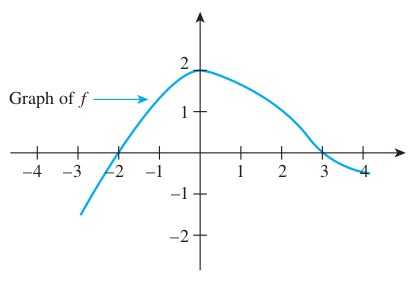
\includegraphics[scale=0.5]{../images/11.1.1.png}
\end{figure}

The graph of a function \(f\) is shown above.

\subsubsection{(a)}
Is \(f(0)\) positive or negative?
\begin{proof}
positive
\end{proof}

\subsubsection{(b)}
For what values of \(x\) does \(f(x) = 0\)?
\begin{proof}
\(f(x) = 0\) when \(x = -2\) and \(x = 3\) (approximately)
\end{proof}

\subsubsection{(c)}
Find approximate values for \(x_1\) and \(x_2\) so that \(f(x_1) = f(x_2) = 1\) but \(x_1 \neq x_2\).
\begin{proof}
\(x_1 = -1\) and \(x_2 = 2\) (approximately)
\end{proof}

\subsubsection{(d)}
Find an approximate value for \(x\) such that \(f(x) = 1.5\).
\begin{proof}
\(x = 1\) or \(x = -1/2\) (approximately)
\end{proof}

\subsubsection{(e)}
As \(x\) increases from \(-3\) to \(-1\), do the values of \(f\) increase or decrease?

\begin{proof}
increase
\end{proof}

\subsubsection{(f)}
As \(x\) increases from 0 to 4, do the values of \(f\) increase or decrease?

\begin{proof}
decrease
\end{proof}

\subsection{Exercise 2}
\begin{figure}[ht!]
\centering
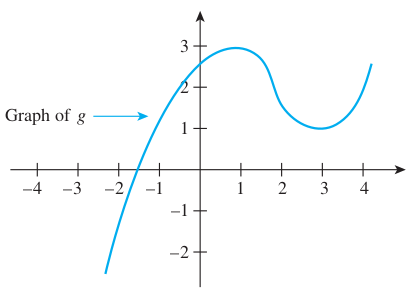
\includegraphics[scale=0.5]{../images/11.1.2.png}
\end{figure}

The graph of a function \(g\) is shown above.

\subsubsection{(a)}
Is \(g(0)\) positive or negative?
\begin{proof}
positive
\end{proof}

\subsubsection{(b)}
Find an approximate value of \(x\) so that \(g(x) = 0\).
\begin{proof}
\(-1.5\) (approximately)
\end{proof}

\subsubsection{(c)}
Find approximate values for \(x_1\) and \(x_2\) so that \(g(x_1) = g(x_2) = 1\) but \(x_1 \neq x_2\).
\begin{proof}
\(x_1 = -1, x_2 = 3\) (approximately)
\end{proof}

\subsubsection{(d)}
Find an approximate value for \(x\) such that \(g(x) = -2\).
\begin{proof}
\(x = -2.2\) (approximately)
\end{proof}

\subsubsection{(e)}
As \(x\) increases from \(-2\) to \(1\), do the values of \(g\) increase or decrease?

\begin{proof}
increase
\end{proof}

\subsubsection{(f)}
As \(x\) increases from 1 to 3, do the values of \(g\) increase or decrease?

\begin{proof}
decrease
\end{proof}

\subsection{Exercise 3}
Sketch the graphs of the power functions \(p_{1/3}\) and \(p_{1/4}\) on the same set of axes. When \(0 < x < 1\), which 
is greater: \(x^{1/3}\) or \(x^{1/4}\)? When \(x > 1\), which is greater: \(x^{1/3}\) or \(x^{1/4}\)?

\begin{proof}
\begin{figure}[ht!]
\centering
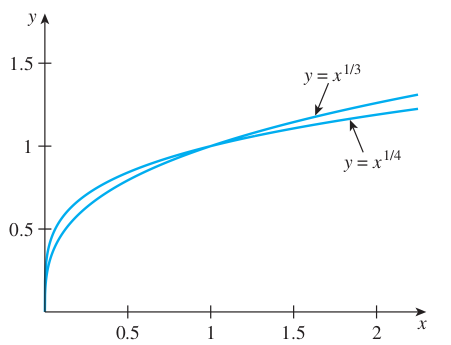
\includegraphics[scale=0.5]{../images/11.1.3.png}
\end{figure}
When \(0 < x < 1\), \(x^{1/3} < x^{1/4}\). When \(1 < x\), \(x^{1/4} < x^{1/3}\).
\end{proof}

\subsection{Exercise 4}
Sketch the graphs of the power functions \(p_3\) and \(p_4\) on the same set of axes. When \(0 < x < 1\), which is greater: 
\(x^3\) or \(x^4\)? When \(x > 1\), which is greater: \(x^3\) or \(x^4\)?

\begin{proof}
\begin{figure}[ht!]
\centering
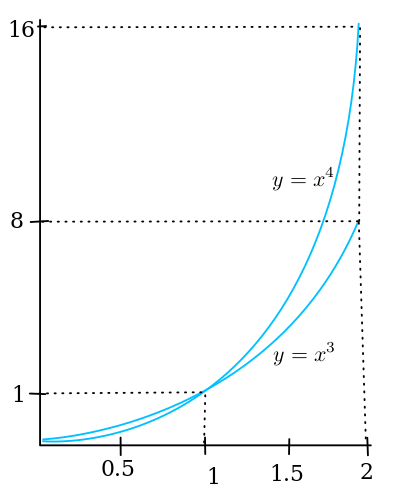
\includegraphics[scale=0.4]{../images/11.1.4.png}
\end{figure}
When \(0 < x < 1\), \(x^4 < x^3\). When \(1 < x\), \(x^3 < x^4\).
\end{proof}

\subsection{Exercise 5}
Sketch the graphs of \(y = 2\floor{x}\); and \(y = \floor{2x}\) for each real number \(x\). What can you conclude from 
these graphs?

\begin{proof}
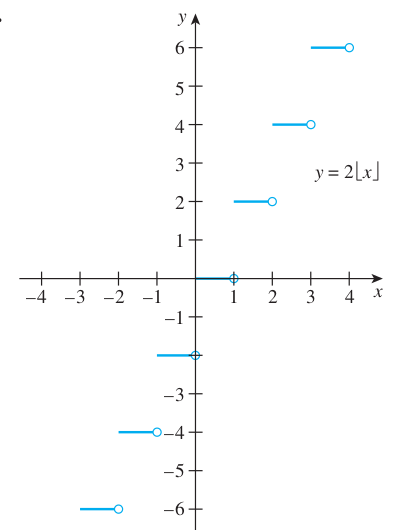
\includegraphics[scale=0.5]{../images/11.1.5.a.png}
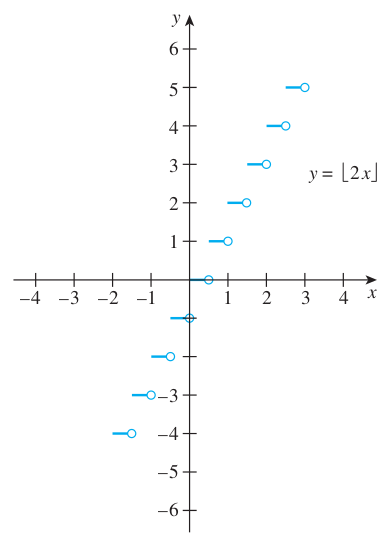
\includegraphics[scale=0.5]{../images/11.1.5.b.png}

The graphs show that \(2\floor{x} \neq \floor{2x}\) for many values of \(x\).
\end{proof}

{\bf \cy Sketch a graph for each of the functions defined in \(6-9\) below.}

\subsection{Exercise 6}
\(g(x) = \ceil{x}\) for each real number \(x\) (Recall that the ceiling of \(x\), \(\ceil{x}\), is the least integer that 
is greater than or equal to \(x\). That is, \(\ceil{x} =\) the unique integer \(n\) such that \(n-1 < x \leq n\).

\begin{proof}
\begin{figure}[ht!]
\centering
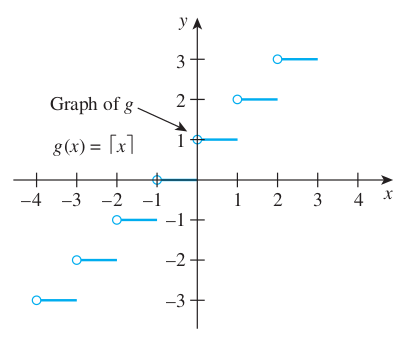
\includegraphics[scale=0.5]{../images/11.1.6.png}
\end{figure}
\end{proof}

\subsection{Exercise 7}
\(h(x) = \ceil{x} - \floor{x}\) for each real number \(x\)

\begin{proof}
\begin{figure}[ht!]
\centering
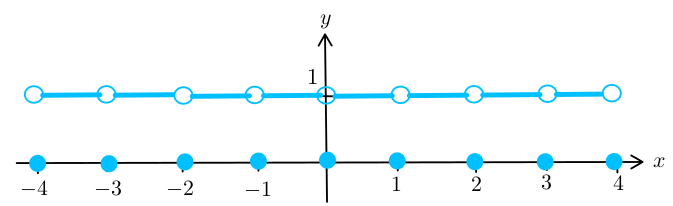
\includegraphics[scale=0.5]{../images/11.1.7.png}
\end{figure}
\end{proof}

\subsection{Exercise 8}
\(F(x) = \floor{x^{1/2}}\) for each real number \(x\)

\begin{proof}
\begin{figure}[ht!]
\centering
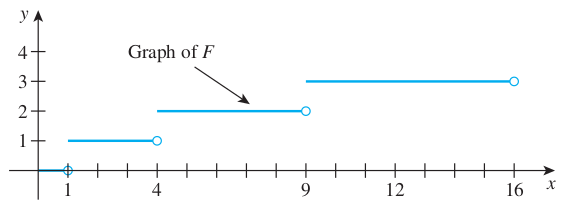
\includegraphics[scale=0.5]{../images/11.1.8.png}
\end{figure}
\end{proof}

\subsection{Exercise 9}
\(G(x) = x - \floor{x}\) for each real number \(x\)

\begin{proof}
\begin{figure}[ht!]
\centering
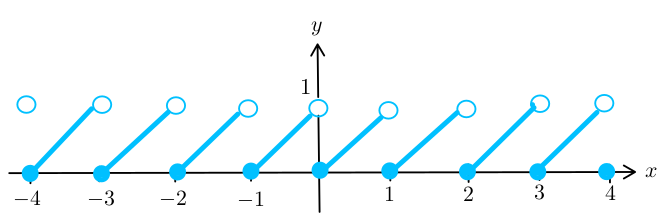
\includegraphics[scale=0.5]{../images/11.1.9.png}
\end{figure}
\end{proof}

{\bf \cy In each of \(10-13\) a function is defined on a set of integers. Sketch a graph for each function.}

\subsection{Exercise 10}
\(f(n) = |n|\) for each integer \(n\)

\begin{proof}
\begin{figure}[ht!]
\centering
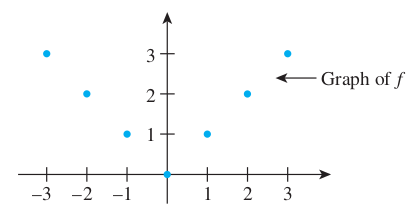
\includegraphics[scale=0.5]{../images/11.1.10.png}
\end{figure}
\end{proof}

\subsection{Exercise 11}
\(g(n) = (n/2) + 1\) for each integer \(n\)

\begin{proof}
\begin{figure}[ht!]
\centering
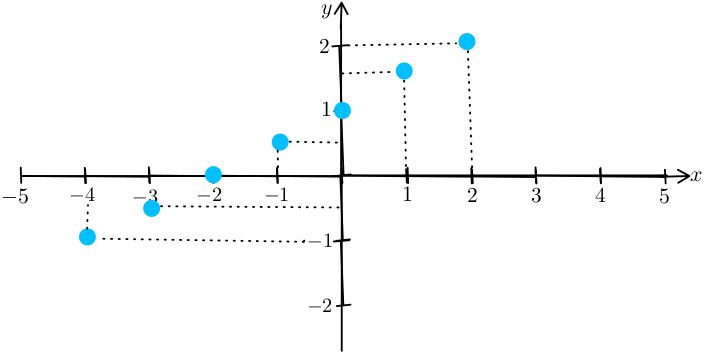
\includegraphics[scale=0.5]{../images/11.1.11.png}
\end{figure}
\end{proof}

\subsection{Exercise 12}
\(h(n) = \floor{n/2}\) for each integer \(n \geq 0\)

\begin{proof}
\begin{figure}[ht!]
\centering
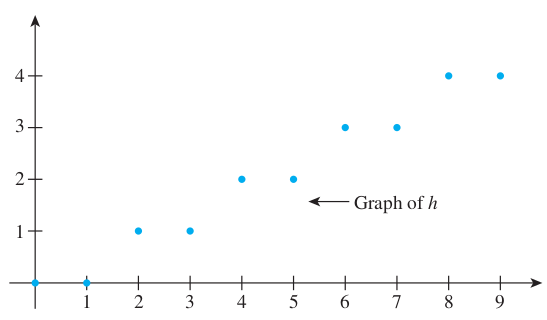
\includegraphics[scale=0.5]{../images/11.1.12.png}
\end{figure}
\end{proof}

\subsection{Exercise 13}
\(k(n) = \floor{n^{1/2}}\) for each integer \(n \geq 0\)

\begin{proof}
\begin{figure}[ht!]
\centering
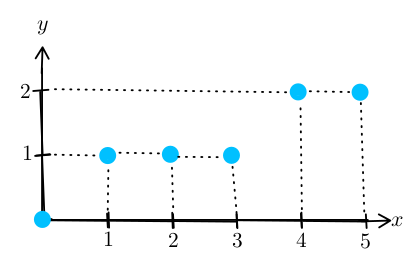
\includegraphics[scale=0.5]{../images/11.1.13.png}
\end{figure}
\end{proof}

\subsection{Exercise 14}
\begin{figure}[ht!]
\centering
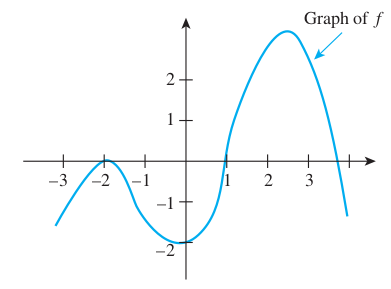
\includegraphics[scale=0.5]{../images/11.1.14.png}
\end{figure}

The graph of a function \(f\) is shown below. Find the intervals on which \(f\) is increasing and the intervals on 
which \(f\) is decreasing.

\begin{proof}
\(f\) is increasing on the intervals \(\{x \in \R \,|\, -3 < x < -2\}\) and \(\{x \in \R \,|\, 0 < x < 2.5\}\), and \(f\) is 
decreasing on \(\{x \in \R \,|\, -2 < x < 0\}\) and \(\{x \in \R \,|\, 2.5 < x < 4\}\) (approximately).
\end{proof}

\subsection{Exercise 15}
Show that the function \(f: \R \to \R\) defined by the formula \(f(x) = 2x - 3\) is increasing on the set of real numbers.

\begin{proof}
Suppose that \(x_1\) and \(x_2\) are particular but arbitrarily chosen real numbers such that \(x_1 < x_2\). 
{\it [We must show that \(f(x_1) < f(x_2)\).]} Since \(x_1 < x_2\) then \(2x_1 < 2x_2\) and \(2x_1 - 3 < 2x_2 - 3\) by 
basic properties of inequalities. Thus, by definition of \(f\), \(f(x_1) < f(x_2)\) {\it [as was to be shown]}. 
Hence \(f\) is increasing on the set of all real numbers.
\end{proof}

\subsection{Exercise 16}
Show that the function \(g: \R \to \R\) defined by the formula \(g(x) = -(x/3) + 1\) is decreasing on the set of real 
numbers.

\begin{proof}

\end{proof}

\subsection{Exercise 17}
Let \(h\) be the function from \(\R\) to \(\R\) defined by the formula \(h(x) = x^2\) for each real number \(x\).

\subsubsection{(a)}
Show that \(h\) is decreasing on the set of real numbers less than zero.

\begin{proof}
Suppose that \(x_1\) and \(x_2\) are particular but arbitrarily chosen real numbers such that \(x_1 < x_2 < 0\). 
{\it [We must show that \(h(x_1) > h(x_2)\).]} 

Since \(x_1 < x_2 < 0\) then \(0 < -x_2 < -x_1\) and multiplying by \(-x_1\) (which is a positive number) we get 
\((-x_1)(-x_2) < (-x_1)(-x_1) = x_1^2\) by basic properties of inequalities. 

Similarly, since \(x_1 < x_2 < 0\) then \(0 < -x_2 < -x_1\) and multiplying by \(-x_2\) (which is a positive number) we 
get \((-x_2)(-x_2) = x_2^2 < (-x_1)(-x_2)\) by basic properties of inequalities. 

By combining the two results we get \(x_2^2 < (-x_1)(-x_2) < x_1^2\) so \(x_2^2 < x_1^2\).

Thus, by definition of \(h\), \(h(x_1) > h(x_2)\) {\it [as was to be shown]}. Hence \(h\) is increasing on the set of all 
real numbers.
\end{proof}

\subsubsection{(b)}
Show that \(h\) is increasing on the set of real numbers greater than zero.

\begin{proof}
Suppose that \(x_1\) and \(x_2\) are particular but arbitrarily chosen real numbers such that \(0 < x_1 < x_2\). 
{\it [We must show that \(h(x_1) < h(x_2)\).]} 

Since \(0 < x_1 < x_2\) then multiplying by \(x_1\) (which is a positive number) we get \(x_1x_1 = x_1^2 < x_1x_2\) by basic 
properties of inequalities. 

Similarly, since \(0 < x_1 < x_2\) then multiplying by \(x_2\) (which is a positive number) we get \(x_1x_2 < x_2x_2 = 
x_2^2\) by basic properties of inequalities. 

By combining the two results we get \(x_1^2 < x_1x_2 < x_2^2\) so \(x_1^2 < x_2^2\).

Thus, by definition of \(h\), \(h(x_1) < h(x_2)\) {\it [as was to be shown]}. Hence \(h\) is increasing on the set of all 
real numbers.
\end{proof}

\subsection{Exercise 18}
Let \(k: \R \to \R\) be the function defined by the formula \(k(x) = (x - 1)/x\) for each real number \(x \neq 0\).

\subsubsection{(a)}
Show that \(k\) is increasing for every real number \(x > 0\).

\begin{proof}
Suppose that \(x_1\) and \(x_2\) are positive real numbers and \(x_1 < x_2\). {\it [We must show that \(k(x_1) < k(x_2)\).]} 

\begin{center}
\begin{tabular}{cll}
& \(x_1 < x_2\) & {\cy by assumption} \\
\(\implies\) & \(-x_2 < -x_1\) & {\cy by multiplying by \(-1\)} \\
\(\implies\) & \(x_1x_2 - x_2 < x_1x_2 - x_1\) & {\cy by adding \(x_1x_2\) to both sides} \\
\(\implies\) & \(x_2(x_1 - 1) < x_1(x_2 - 1)\) & {\cy by factoring both sides} \\
\(\implies\) & \(\dps \frac{x_1 - 1}{x_1} < \frac{x_2 - 1}{x_2}\) & {\cy by dividing both sides by \(x_1x_2 > 0\)} \\
\(\implies\) & \(k(x_1) < k(x_2)\) & {\cy by definition of \(k\)}
\end{tabular}
\end{center}

\end{proof}

\subsubsection{(b)}
Is \(k\) increasing or decreasing for \(x < 0\)? Prove your answer.

\begin{proof}
It is increasing. The same proof as in part (a) works. Note that the only place in the proof where the signs of \(x_1\)
and \(x_2\) matter is when we divide both sides by \(x_1x_2\). For the proof to work, \(x_1x_2\) has to be positive. But if
both \(x_1\) and \(x_2\) are negative, then \(x_1x_2\) {\it is} positive. Therefore the proof still works.
\end{proof}

\subsection{Exercise 19}
Show that if a function \(f: \R \to \R\) is increasing, then \(f\) is one-to-one.

\begin{proof}
Suppose \(f: \R \to \R\) is increasing. {\it [We must show that \(f\) is one-to-one. In other words, we must show that 
for all real numbers \(x_1\) and \(x_2\) , if \(x_1 \neq x_2\) then \(f(x_1) = f(x_2)\).]} Suppose \(x_1\) and \(x_2\) are 
real numbers and \(x_1 \neq x_2\). By the trichotomy law {\it [Appendix A, T17]} \(x_1 < x2\), or \(x_1 > x_2\). In case 
\(x_1 < x_2\), then since \(f\) is increasing, \(f(x_1) < f(x_2)\) and so \(f(x_1) \neq f(x_2)\). Similarly, in case 
\(x_1 > x_2\), then \(f(x_1) > f(x_2)\) and so \(f(x_1)\neq f(x_2)\). Thus in either case, \(f(x_1) \neq f(x_2)\) 
{\it [as was to be shown].}
\end{proof}

\subsection{Exercise 20}
Given real-valued functions \(f\) and \(g\) with the same domain \(D\), the sum of \(f\) and \(g\), denoted \(f + g\), 
is defined as follows: For each real number \(x\), \((f + g)(x) = f(x) + g(x)\). Show that if \(f\) and \(g\) are both 
increasing on a set \(S\), then \(f + g\) is also increasing on \(S\).

\begin{proof}
Assume \(x_1, x_2 \in S\) and \(x_1 < x_2\). {\it [We want to show \((f+g)(x_1) < (f+g)(x_2)\).]} Since \(f\) is increasing,
\(f(x_1) < f(x_2)\). Since \(g\) is increasing, \(g(x_1) < g(x_2)\). By definition of \(f+g\) we have \((f+g)(x_1) = 
f(x_1) + g(x_1) < f(x_2) + g(x_2) = (f+g)(x_2)\), {\it [as was to be shown.]}
\end{proof}

\subsection{Exercise 21}
\subsubsection{(a)}
Let \(m\) be any positive integer, and define \(f(x) = x^m\) for each nonnegative real number \(x\). Use the binomial 
theorem to show that \(f\) is an increasing function.

\begin{proof}
Suppose \(u\) and \(v\) are nonnegative real numbers with \(u < v\). {\it [We must show that \(f(u) < f(v)\).]} Note that 
\(v = u + h\) for some positive real number \(h\). By substitution and the binomial theorem,
\[
v^m = (u+h)^m = \sum_{i = 0}^{m}\binom{m}{i} u^{m-i} h^i = u^m + \sum_{i = 1}^{m}\binom{m}{i} u^{m-i} h^i
\]
The last summation is positive because \(u \geq 0\) and \(h > 0\), and a sum of nonnegative terms that includes at least one 
positive term is positive. Hence \(v^m = u^m +\) a positive number, and so \(f(u) = u^m < v^m = f(v)\),
{\it [as was to be shown]}.
\end{proof}

\subsubsection{(b)}
Let \(m\) and \(n\) be any positive integers, and let \(g(x) = x^{m/n}\) for each nonnegative real number \(x\). Prove that 
\(g\) is an increasing function. 

{\it Note: The results of exercise 21 are used in the exercises for Sections 11.2 and 11.4.}

\begin{proof}
Write \(f(x) = x^m\). Then \(g(x) = (f(x))^{1/n}\) by the law of exponents. 

Now assume \(0 \leq x_1 < x_2\). In part (a) we showed that \(f\) is increasing. Therefore \(f(x_1) < f(x_2)\), in other 
words \(x_1^m < x_2^m\). So we need to show that the function \(h(x) = x^{1/n}\) is an increasing function. That will imply
\(g(x_1) = h(x_1^m) < h(x_2^m) = g(x_2)\), in other words \(x_1^{m/n} < x_2^{m/n}\), which is what we want.

To show \(h\) is increasing, assume \(0 \leq z_1 < z_2\). By definition, \(h(z_1) = z_1^{1/n} = y_1\) is the real number
with the property that \(y_1^n = z_1\). Similarly \(h(z_2) = z_2^{1/n} = y_2\) is the real number with the property that 
\(y_2^n = z_2\). {\it [We want to show \(y_1 < y_2\).]}

Argue by contradiction and assume \(y_2 \leq y_1\). Now consider the function \(e(y) = y^n\). This function is also
increasing by part (a), since \(m\) and \(n\) are both any positive integers. Therefore \(e(y_2) \leq e(y_1)\), in other
words \(z_2 \leq z_1\), which is a contradiction!

Therefore \(y_1 < y_2\) and \(h\) is increasing, and thus \(g\) is increasing as a consequence.
\end{proof}

\subsection{Exercise 22}
\begin{figure}[ht!]
\centering
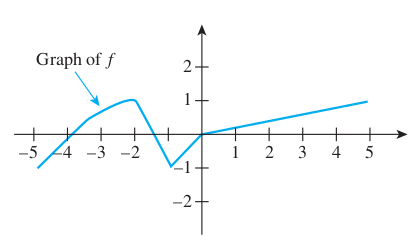
\includegraphics[scale=0.5]{../images/11.1.22.png}
\end{figure}

Let \(f\) be the function whose graph follows. Sketch the graph of \(3f\).

\begin{proof}
\begin{figure}[ht!]
\centering
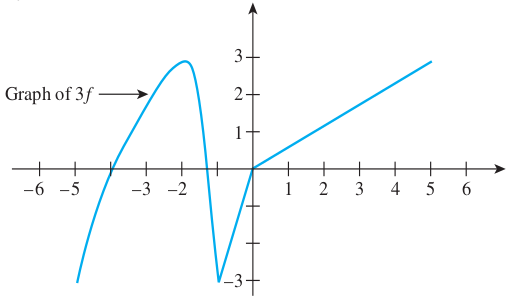
\includegraphics[scale=0.5]{../images/11.1.22.2.png}
\end{figure}
\end{proof}

\subsection{Exercise 23}
\begin{figure}[ht!]
\centering
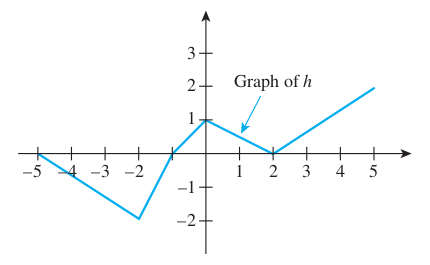
\includegraphics[scale=0.5]{../images/11.1.23.png}
\end{figure}

Let \(h\) be the function whose graph is shown above. Sketch the graph of \(2h\).

\begin{proof}
\begin{figure}[ht!]
\centering
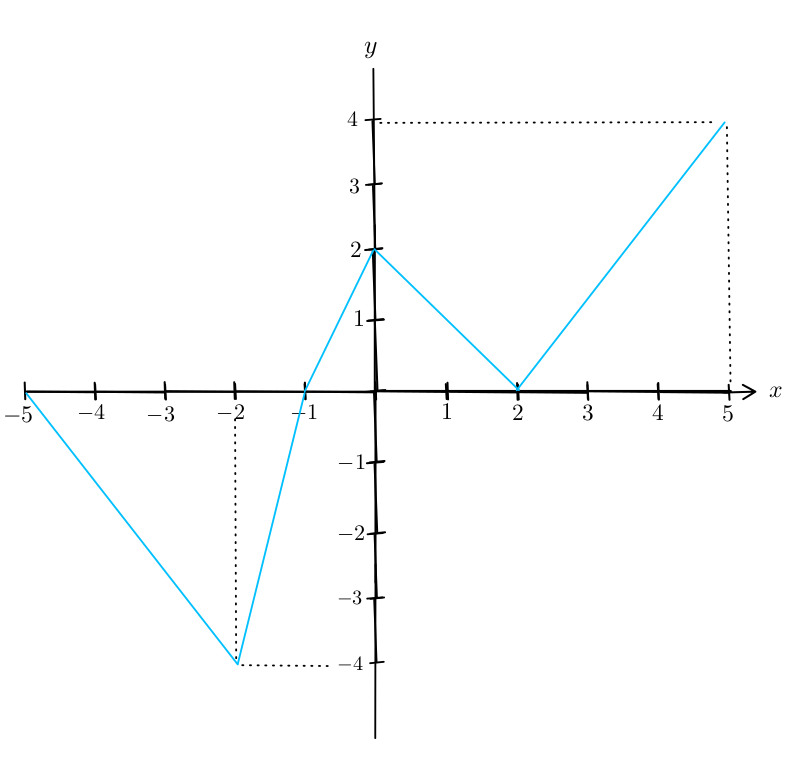
\includegraphics[scale=0.3]{../images/11.1.23.2.png}
\end{figure}
\end{proof}

\subsection{Exercise 24}
Let \(f\) be a real-valued function of a real variable. Show that if \(f\) is decreasing on a set \(S\) and if \(M\) is any 
positive real number, then \(Mf\) is decreasing on \(S\).

\begin{proof}
Suppose that \(f\) is a real-valued function of a real variable, \(f\) is decreasing on a set \(S\), and \(M\) is any 
positive real number. {\it [We must show that \(Mf\) is decreasing on \(S\). In other words, we must show that for all 
\(x_1\) and \(x_2\) in \(S\), if \(x_1 < x_2\) then \((Mf)(x_1) > (Mf)(x_2)\).]} Suppose \(x_1\) and \(x_2\) are in 
\(S\) and \(x_1 < x_2\). Since \(f\) is decreasing on \(S\), \(f(x_1) > f(x_2)\), and since \(M\) is positive, \(Mf(x_1) >
Mf(x_2)\) {\it [because when both sides of an inequality are multiplied by a positive number, the direction of the 
inequality is unchanged].} It follows by definition of \(Mf\) that \((Mf)(x_1) > (Mf)(x_2)\), {\it [as was to be shown].}
\end{proof}

\subsection{Exercise 25}
Let \(f\) be a real-valued function of a real variable. Show that if \(f\) is increasing on a set \(S\) and if \(M\) is any 
negative real number, then \(Mf\) is decreasing on \(S\).

\begin{proof}
The proof is the same as in Exercise 24, except that this time we have \(f(x_1) < f(x_2)\) because \(f\) is increasing, and 
multiplying an inequality by a negative number \(M\) reverses
the direction of the equality, so \(Mf(x_1) > Mf(x_2)\).
\end{proof}

\subsection{Exercise 26}
Let \(f\) be a real-valued function of a real variable. Show that if \(f\) is decreasing on a set \(S\) and if \(M\) is any 
negative real number, then \(Mf\) is increasing on \(S\).

\begin{proof}
The proof is the same as in Exercise 24, except that this time 
multiplying an inequality by a negative number \(M\) reverses
the direction of the equality, so \(Mf(x_1) < Mf(x_2)\).
\end{proof}

{\bf \cy In 27 and 28, functions \(f\) and \(g\) are defined. In each case sketch the graphs of \(f\) and \(2g\) on the same 
set of axes and find a number \(x_0\) so that \(f(x) \leq 2g(x)\) for all \(x > x_0\). You can find an exact value for 
\(x_0\) by solving a quadratic equation, or you can find an approximate value for \(x_0\) by using a graphing calculator 
or computer.}

\subsection{Exercise 27}
\(f(x) = x^2 + 10x + 11\) and \(g(x) = x^2\) for each real number \(x \geq 0\)

\begin{proof}
\begin{figure}[ht!]
\centering
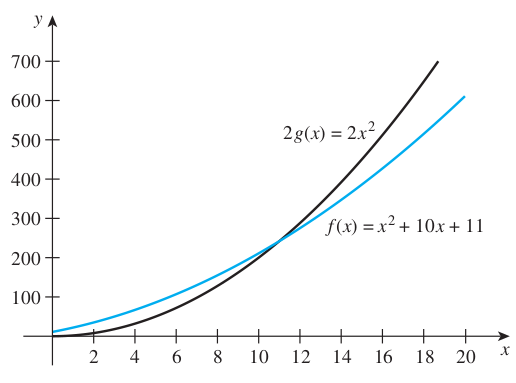
\includegraphics[scale=0.5]{../images/11.1.27.png}
\end{figure}

To find the answer algebraically, solve the equation \(2x^2 = x^2 + 10x + 11\) for \(x\). Subtracting \(x^2\) from both 
sides gives \(x^2 - 10x - 11 = 0\), and either using the quadratic formula or factoring \(x^2-10x-11=(x - 11)(x + 1)\) 
gives \(x = 11\) (since \(x > 0\)). To find an approximate answer with a graphing calculator, plot both \(f(x) = x^2 + 
10x + 11\) and \(2g(x) = 2x^2\) for \(x > 0\), as shown in the figure, and find that \(2g(x) > f(x)\) when \(x > 11\) 
(approximately). You can obtain only an approximate answer from a graphing calculator because the calculator computes 
values only to an accuracy of a finite number of decimal places.
\end{proof}

\subsection{Exercise 28}
\(f(x) = x^2 + 125x + 254\) and \(g(x) = x^2\) for each real number \(x \geq 0\)

\begin{proof}
\begin{figure}[ht!]
\centering
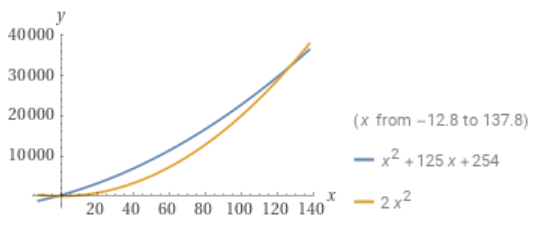
\includegraphics[scale=0.5]{../images/11.1.28.png}
\end{figure}
If we set \(f(x) = 2g(x)\) and solve, we get \(x^2 + 125x + 254 = 2x^2\) which gives \(x^2 - 125x - 254 = 0\) which 
factors as \((x-127)(x+2) = 0\) which has solutions \(x = -2, 127\). So let \(x_0 = 127\), so that \(f(x) < g(x)\) for all
\(x > x_0 = 127\).
\end{proof}

\section{Exercise Set 11.2}

\subsection{Exercise 1}

\subsubsection{()}

\begin{proof}

\end{proof}

\subsection{Exercise 2}

\subsubsection{()}

\begin{proof}

\end{proof}

\subsection{Exercise 3}

\subsubsection{()}

\begin{proof}

\end{proof}

\subsection{Exercise 4}

\subsubsection{()}

\begin{proof}

\end{proof}

\subsection{Exercise 5}

\subsubsection{()}

\begin{proof}

\end{proof}

\subsection{Exercise 6}

\subsubsection{()}

\begin{proof}

\end{proof}

\subsection{Exercise 7}

\subsubsection{()}

\begin{proof}

\end{proof}

\subsection{Exercise 8}

\subsubsection{()}

\begin{proof}

\end{proof}

\subsection{Exercise 9}

\subsubsection{()}

\begin{proof}

\end{proof}

\subsection{Exercise 10}

\subsubsection{()}

\begin{proof}

\end{proof}

\subsection{Exercise 11}

\subsubsection{()}

\begin{proof}

\end{proof}

\subsection{Exercise 12}

\subsubsection{()}

\begin{proof}

\end{proof}

\subsection{Exercise 13}

\subsubsection{()}

\begin{proof}

\end{proof}

\subsection{Exercise 14}

\subsubsection{()}

\begin{proof}

\end{proof}

\subsection{Exercise 15}

\subsubsection{()}

\begin{proof}

\end{proof}

\subsection{Exercise 16}

\subsubsection{()}

\begin{proof}

\end{proof}

\subsection{Exercise 17}

\subsubsection{()}

\begin{proof}

\end{proof}

\subsection{Exercise 18}

\subsubsection{()}

\begin{proof}

\end{proof}

\subsection{Exercise 19}

\subsubsection{()}

\begin{proof}

\end{proof}

\subsection{Exercise 20}

\subsubsection{()}

\begin{proof}

\end{proof}

\subsection{Exercise 21}

\subsubsection{()}

\begin{proof}

\end{proof}

\subsection{Exercise 22}

\subsubsection{()}

\begin{proof}

\end{proof}

\subsection{Exercise 23}

\subsubsection{()}

\begin{proof}

\end{proof}

\subsection{Exercise 24}

\subsubsection{()}

\begin{proof}

\end{proof}

\subsection{Exercise 25}

\subsubsection{()}

\begin{proof}

\end{proof}

\subsection{Exercise 26}

\subsubsection{()}

\begin{proof}

\end{proof}

\subsection{Exercise 27}

\subsubsection{()}

\begin{proof}

\end{proof}

\subsection{Exercise 28}

\subsubsection{()}

\begin{proof}

\end{proof}

\subsection{Exercise 29}

\subsubsection{()}

\begin{proof}

\end{proof}

\subsection{Exercise 30}

\subsubsection{()}

\begin{proof}

\end{proof}

\subsection{Exercise 31}

\subsubsection{()}

\begin{proof}

\end{proof}

\subsection{Exercise 32}

\subsubsection{()}

\begin{proof}

\end{proof}

\subsection{Exercise 33}

\subsubsection{()}

\begin{proof}

\end{proof}

\subsection{Exercise 34}

\subsubsection{()}

\begin{proof}

\end{proof}

\subsection{Exercise 35}

\subsubsection{()}

\begin{proof}

\end{proof}

\subsection{Exercise 36}

\subsubsection{()}

\begin{proof}

\end{proof}

\subsection{Exercise 37}

\subsubsection{()}

\begin{proof}

\end{proof}

\subsection{Exercise 38}

\subsubsection{()}

\begin{proof}

\end{proof}

\subsection{Exercise 39}

\subsubsection{()}

\begin{proof}

\end{proof}

\subsection{Exercise 40}

\subsubsection{()}

\begin{proof}

\end{proof}

\subsection{Exercise 41}

\subsubsection{()}

\begin{proof}

\end{proof}

\subsection{Exercise 42}

\subsubsection{()}

\begin{proof}

\end{proof}

\subsection{Exercise 43}

\subsubsection{()}

\begin{proof}

\end{proof}

\subsection{Exercise 44}

\subsubsection{()}

\begin{proof}

\end{proof}

\subsection{Exercise 45}

\subsubsection{()}

\begin{proof}

\end{proof}

\subsection{Exercise 46}

\subsubsection{()}

\begin{proof}

\end{proof}

\subsection{Exercise 47}

\subsubsection{()}

\begin{proof}

\end{proof}

\subsection{Exercise 48}

\subsubsection{()}

\begin{proof}

\end{proof}

\subsection{Exercise 49}

\subsubsection{()}

\begin{proof}

\end{proof}

\subsection{Exercise 50}

\subsubsection{()}

\begin{proof}

\end{proof}

\subsection{Exercise 51}

\subsubsection{()}

\begin{proof}

\end{proof}

\section{Exercise Set 11.3}

\subsection{Exercise 1}

\subsubsection{()}

\begin{proof}

\end{proof}

\subsection{Exercise 2}

\subsubsection{()}

\begin{proof}

\end{proof}

\subsection{Exercise 3}

\subsubsection{()}

\begin{proof}

\end{proof}

\subsection{Exercise 4}

\subsubsection{()}

\begin{proof}

\end{proof}

\subsection{Exercise 5}

\subsubsection{()}

\begin{proof}

\end{proof}

\subsection{Exercise 6}

\subsubsection{()}

\begin{proof}

\end{proof}

\subsection{Exercise 7}

\subsubsection{()}

\begin{proof}

\end{proof}

\subsection{Exercise 8}

\subsubsection{()}

\begin{proof}

\end{proof}

\subsection{Exercise 9}

\subsubsection{()}

\begin{proof}

\end{proof}

\subsection{Exercise 10}

\subsubsection{()}

\begin{proof}

\end{proof}

\subsection{Exercise 11}

\subsubsection{()}

\begin{proof}

\end{proof}

\subsection{Exercise 12}

\subsubsection{()}

\begin{proof}

\end{proof}

\subsection{Exercise 13}

\subsubsection{()}

\begin{proof}

\end{proof}

\subsection{Exercise 14}

\subsubsection{()}

\begin{proof}

\end{proof}

\subsection{Exercise 15}

\subsubsection{()}

\begin{proof}

\end{proof}

\subsection{Exercise 16}

\subsubsection{()}

\begin{proof}

\end{proof}

\subsection{Exercise 17}

\subsubsection{()}

\begin{proof}

\end{proof}

\subsection{Exercise 18}

\subsubsection{()}

\begin{proof}

\end{proof}

\subsection{Exercise 19}

\subsubsection{()}

\begin{proof}

\end{proof}

\subsection{Exercise 20}

\subsubsection{()}

\begin{proof}

\end{proof}

\subsection{Exercise 21}

\subsubsection{()}

\begin{proof}

\end{proof}

\subsection{Exercise 22}

\subsubsection{()}

\begin{proof}

\end{proof}

\subsection{Exercise 23}

\subsubsection{()}

\begin{proof}

\end{proof}

\subsection{Exercise 24}

\subsubsection{()}

\begin{proof}

\end{proof}

\subsection{Exercise 25}

\subsubsection{()}

\begin{proof}

\end{proof}

\subsection{Exercise 26}

\subsubsection{()}

\begin{proof}

\end{proof}

\subsection{Exercise 27}

\subsubsection{()}

\begin{proof}

\end{proof}

\subsection{Exercise 28}

\subsubsection{()}

\begin{proof}

\end{proof}

\subsection{Exercise 29}

\subsubsection{()}

\begin{proof}

\end{proof}

\subsection{Exercise 30}

\subsubsection{()}

\begin{proof}

\end{proof}

\subsection{Exercise 31}

\subsubsection{()}

\begin{proof}

\end{proof}

\subsection{Exercise 32}

\subsubsection{()}

\begin{proof}

\end{proof}

\subsection{Exercise 33}

\subsubsection{()}

\begin{proof}

\end{proof}

\subsection{Exercise 34}

\subsubsection{()}

\begin{proof}

\end{proof}

\subsection{Exercise 35}

\subsubsection{()}

\begin{proof}

\end{proof}

\subsection{Exercise 36}

\subsubsection{()}

\begin{proof}

\end{proof}

\subsection{Exercise 37}

\subsubsection{()}

\begin{proof}

\end{proof}

\subsection{Exercise 38}

\subsubsection{()}

\begin{proof}

\end{proof}

\subsection{Exercise 39}

\subsubsection{()}

\begin{proof}

\end{proof}

\subsection{Exercise 40}

\subsubsection{()}

\begin{proof}

\end{proof}

\subsection{Exercise 41}

\subsubsection{()}

\begin{proof}

\end{proof}

\subsection{Exercise 42}

\subsubsection{()}

\begin{proof}

\end{proof}

\subsection{Exercise 43}

\subsubsection{()}

\begin{proof}

\end{proof}

\section{Exercise Set 11.4}

\subsection{Exercise 1}

\subsubsection{()}

\begin{proof}

\end{proof}

\subsection{Exercise 2}

\subsubsection{()}

\begin{proof}

\end{proof}

\subsection{Exercise 3}

\subsubsection{()}

\begin{proof}

\end{proof}

\subsection{Exercise 4}

\subsubsection{()}

\begin{proof}

\end{proof}

\subsection{Exercise 5}

\subsubsection{()}

\begin{proof}

\end{proof}

\subsection{Exercise 6}

\subsubsection{()}

\begin{proof}

\end{proof}

\subsection{Exercise 7}

\subsubsection{()}

\begin{proof}

\end{proof}

\subsection{Exercise 8}

\subsubsection{()}

\begin{proof}

\end{proof}

\subsection{Exercise 9}

\subsubsection{()}

\begin{proof}

\end{proof}

\subsection{Exercise 10}

\subsubsection{()}

\begin{proof}

\end{proof}

\subsection{Exercise 11}

\subsubsection{()}

\begin{proof}

\end{proof}

\subsection{Exercise 12}

\subsubsection{()}

\begin{proof}

\end{proof}

\subsection{Exercise 13}

\subsubsection{()}

\begin{proof}

\end{proof}

\subsection{Exercise 14}

\subsubsection{()}

\begin{proof}

\end{proof}

\subsection{Exercise 15}

\subsubsection{()}

\begin{proof}

\end{proof}

\subsection{Exercise 16}

\subsubsection{()}

\begin{proof}

\end{proof}

\subsection{Exercise 17}

\subsubsection{()}

\begin{proof}

\end{proof}

\subsection{Exercise 18}

\subsubsection{()}

\begin{proof}

\end{proof}

\subsection{Exercise 19}

\subsubsection{()}

\begin{proof}

\end{proof}

\subsection{Exercise 20}

\subsubsection{()}

\begin{proof}

\end{proof}

\subsection{Exercise 21}

\subsubsection{()}

\begin{proof}

\end{proof}

\subsection{Exercise 22}

\subsubsection{()}

\begin{proof}

\end{proof}

\subsection{Exercise 23}

\subsubsection{()}

\begin{proof}

\end{proof}

\subsection{Exercise 24}

\subsubsection{()}

\begin{proof}

\end{proof}

\subsection{Exercise 25}

\subsubsection{()}

\begin{proof}

\end{proof}

\subsection{Exercise 26}

\subsubsection{()}

\begin{proof}

\end{proof}

\subsection{Exercise 27}

\subsubsection{()}

\begin{proof}

\end{proof}

\subsection{Exercise 28}

\subsubsection{()}

\begin{proof}

\end{proof}

\subsection{Exercise 29}

\subsubsection{()}

\begin{proof}

\end{proof}

\subsection{Exercise 30}

\subsubsection{()}

\begin{proof}

\end{proof}

\subsection{Exercise 31}

\subsubsection{()}

\begin{proof}

\end{proof}

\subsection{Exercise 32}

\subsubsection{()}

\begin{proof}

\end{proof}

\subsection{Exercise 33}

\subsubsection{()}

\begin{proof}

\end{proof}

\subsection{Exercise 34}

\subsubsection{()}

\begin{proof}

\end{proof}

\subsection{Exercise 35}

\subsubsection{()}

\begin{proof}

\end{proof}

\subsection{Exercise 36}

\subsubsection{()}

\begin{proof}

\end{proof}

\subsection{Exercise 37}

\subsubsection{()}

\begin{proof}

\end{proof}

\subsection{Exercise 38}

\subsubsection{()}

\begin{proof}

\end{proof}

\subsection{Exercise 39}

\subsubsection{()}

\begin{proof}

\end{proof}

\subsection{Exercise 40}

\subsubsection{()}

\begin{proof}

\end{proof}

\subsection{Exercise 41}

\subsubsection{()}

\begin{proof}

\end{proof}

\subsection{Exercise 42}

\subsubsection{()}

\begin{proof}

\end{proof}

\subsection{Exercise 43}

\subsubsection{()}

\begin{proof}

\end{proof}

\subsection{Exercise 44}

\subsubsection{()}

\begin{proof}

\end{proof}

\subsection{Exercise 45}

\subsubsection{()}

\begin{proof}

\end{proof}

\subsection{Exercise 46}

\subsubsection{()}

\begin{proof}

\end{proof}

\subsection{Exercise 47}

\subsubsection{()}

\begin{proof}

\end{proof}

\subsection{Exercise 48}

\subsubsection{()}

\begin{proof}

\end{proof}

\subsection{Exercise 49}

\subsubsection{()}

\begin{proof}

\end{proof}

\subsection{Exercise 50}

\subsubsection{()}

\begin{proof}

\end{proof}

\subsection{Exercise 51}

\subsubsection{()}

\begin{proof}

\end{proof}

\section{Exercise Set 11.5}

\subsection{Exercise 1}

\subsubsection{()}

\begin{proof}

\end{proof}

\subsection{Exercise 2}

\subsubsection{()}

\begin{proof}

\end{proof}

\subsection{Exercise 3}

\subsubsection{()}

\begin{proof}

\end{proof}

\subsection{Exercise 4}

\subsubsection{()}

\begin{proof}

\end{proof}

\subsection{Exercise 5}

\subsubsection{()}

\begin{proof}

\end{proof}

\subsection{Exercise 6}

\subsubsection{()}

\begin{proof}

\end{proof}

\subsection{Exercise 7}

\subsubsection{()}

\begin{proof}

\end{proof}

\subsection{Exercise 8}

\subsubsection{()}

\begin{proof}

\end{proof}

\subsection{Exercise 9}

\subsubsection{()}

\begin{proof}

\end{proof}

\subsection{Exercise 10}

\subsubsection{()}

\begin{proof}

\end{proof}

\subsection{Exercise 11}

\subsubsection{()}

\begin{proof}

\end{proof}

\subsection{Exercise 12}

\subsubsection{()}

\begin{proof}

\end{proof}

\subsection{Exercise 13}

\subsubsection{()}

\begin{proof}

\end{proof}

\subsection{Exercise 14}

\subsubsection{()}

\begin{proof}

\end{proof}

\subsection{Exercise 15}

\subsubsection{()}

\begin{proof}

\end{proof}

\subsection{Exercise 16}

\subsubsection{()}

\begin{proof}

\end{proof}

\subsection{Exercise 17}

\subsubsection{()}

\begin{proof}

\end{proof}

\subsection{Exercise 18}

\subsubsection{()}

\begin{proof}

\end{proof}

\subsection{Exercise 19}

\subsubsection{()}

\begin{proof}

\end{proof}

\subsection{Exercise 20}

\subsubsection{()}

\begin{proof}

\end{proof}

\subsection{Exercise 21}

\subsubsection{()}

\begin{proof}

\end{proof}

\subsection{Exercise 22}

\subsubsection{()}

\begin{proof}

\end{proof}

\subsection{Exercise 23}

\subsubsection{()}

\begin{proof}

\end{proof}

\subsection{Exercise 24}

\subsubsection{()}

\begin{proof}

\end{proof}

\subsection{Exercise 25}

\subsubsection{()}

\begin{proof}

\end{proof}

\subsection{Exercise 26}

\subsubsection{()}

\begin{proof}

\end{proof}

\end{document}
